\chapter{Experiments}
\section{Dataset Preparation}
After the selection of our Dataset which is IStego100K\cite{7}, now we need to further process this dataset. It was not feasible to train the model using all data at once. So, Initially we splitted the dataset into different batches. Each batch consisting of 40,000 images (20000 cover images and 20000 stego images). We tried to train the model using this subset of datset but there was mermory Limitation problem. We then reduced the batch size to 30,000 (15,000 cover images and 15,000 stego images), but still faced the same issue. Finally, we set the batch size to 20,000 (10,000 cover and 10,000 stego), which allowed the training process to proceed successfully. To split the dataset, we utilized a Microsoft PowerShell script, which splitted the dataset into the desired subsets and stored them in respective subfolders.

\section{Trainig the Ensemble Model}
Before training the model, it was necessary to identify the most suitable features for our project. Therefore, we conducted several tests to determine the optimal feature set for training our model.
\subsection{DCTR Feature}
Initially, we used (DCTR) features with a feature dimensionality of 8000 for training our model. However, we faced several challenges: the feature extraction process was time-consuming, and the outcomes were unsatisfactory.\\
\begin{figure}[H]
    \begin{subfigure}[b]{0.5\textwidth}
        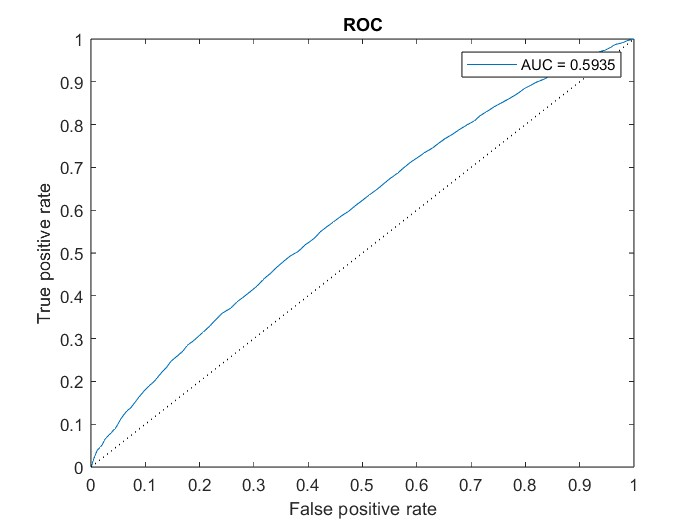
\includegraphics[width=\textwidth]{img/rocdctr.jpg}
    \end{subfigure}
    \hfill
    \begin{subfigure}[b]{0.5\textwidth}
        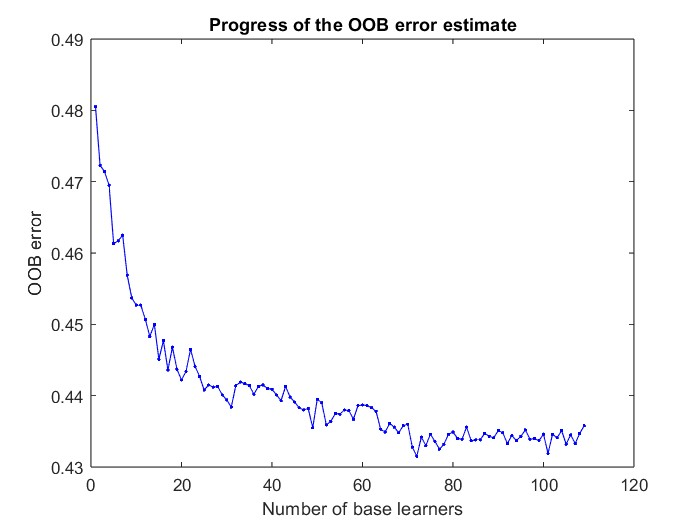
\includegraphics[width=\textwidth]{img/saturationdctr.jpg}
    \end{subfigure}
    \caption{ROC and Search for subspace dimensionality}
\end{figure}
\begin{figure}[H]
    \begin{subfigure}[b]{0.5\textwidth}
        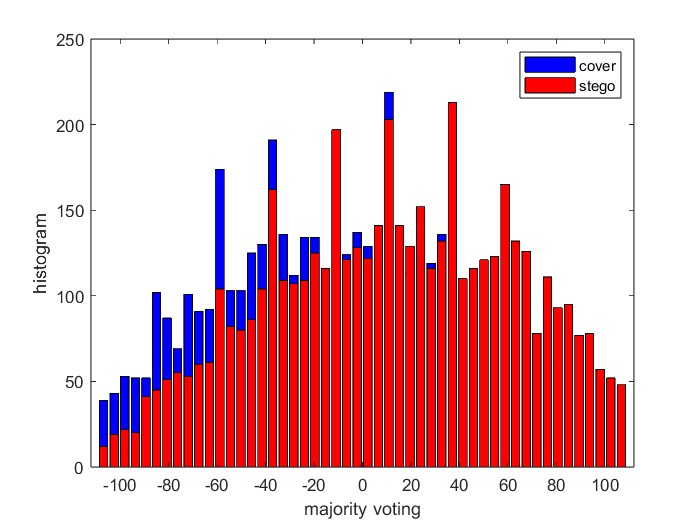
\includegraphics[width=\textwidth]{img/histoDctr.jpg}
    \end{subfigure}
    \hfill
    \begin{subfigure}[b]{0.5\textwidth}
        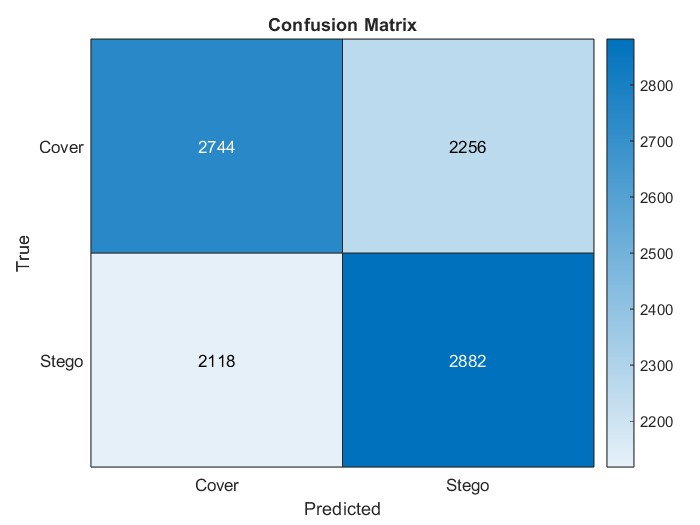
\includegraphics[width=\textwidth]{img/confusiondctr.jpg}
    \end{subfigure}
    \caption{Histogram and Confusion Matrix}
\end{figure}
\clearpage
\subsection{CC-CN Feature}
Later on, we came across cc-cN features, specifically cc-c300, which provided a higher dimensionality of 48600. These features proved to be more effective in capturing dependencies among individual cover elements. Due to the large dimensionality of our images, we used for Fisher's Linear Discriminant (FLD) as the base learner for our ensemble classifier. As a result, we observed improved performance compared to our earlier one.\\
\begin{figure}[H]
    \begin{subfigure}[b]{0.5\textwidth}
        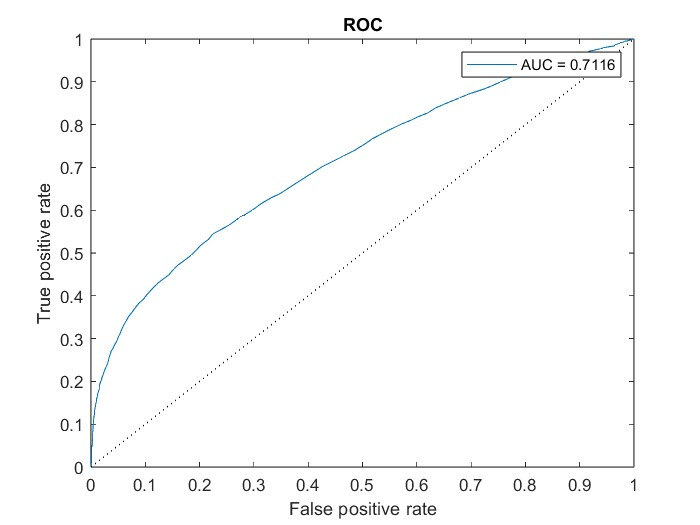
\includegraphics[width=\textwidth]{img/ROC300.jpg}
    \end{subfigure}
    \hfill
    \begin{subfigure}[b]{0.5\textwidth}
        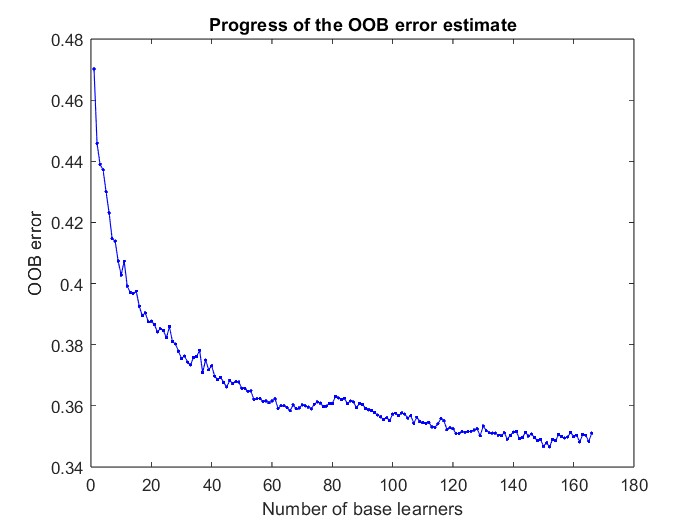
\includegraphics[width=\textwidth]{img/saturation300.jpg}
    \end{subfigure}
    \caption{ROC and Search for subspace dimensionality}
\end{figure}
\begin{figure}[H]
    \begin{subfigure}[b]{0.5\textwidth}
        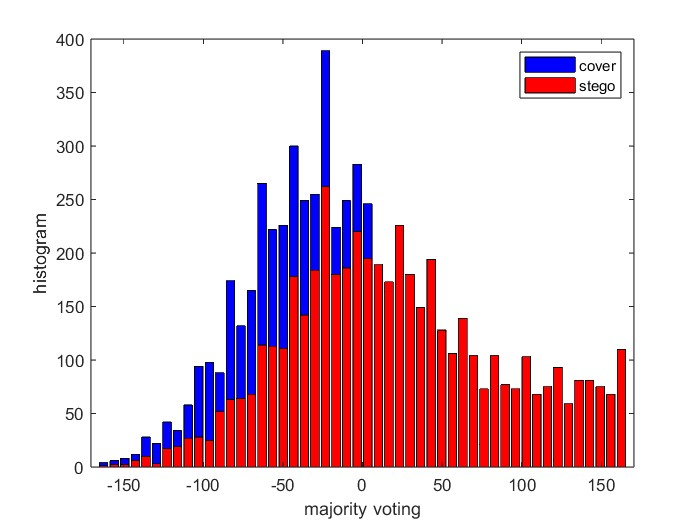
\includegraphics[width=\textwidth]{img/histo300.jpg}
    \end{subfigure}
    \hfill
    \begin{subfigure}[b]{0.5\textwidth}
        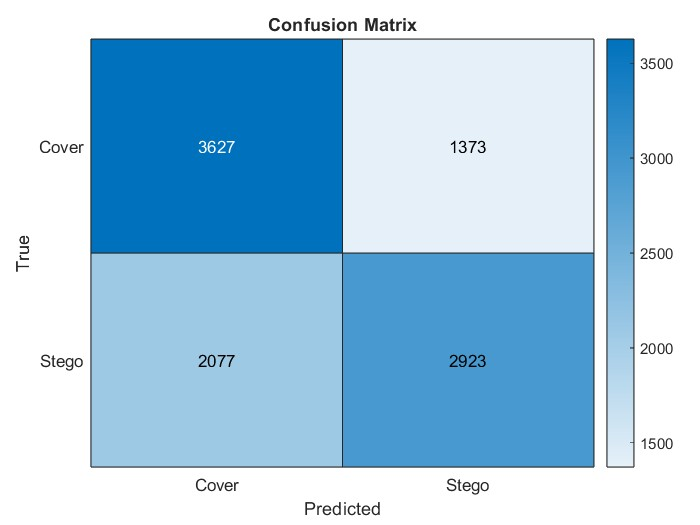
\includegraphics[width=\textwidth]{img/confusion300.jpg}
    \end{subfigure}
    \caption{Histogram and Confusion Matrix}
\end{figure}
\clearpage
\subsection{CC-CHEN Feature}
We looked into another feature extraction method called cc-chen, which had 972 dimensions, to see if it was better than cc-c300. However, the results weren't as good as with cc-c300. So, we decided that cc-c300 was the best choice for our project.\\
\begin{figure}[H]
    \begin{subfigure}[b]{0.5\textwidth}
        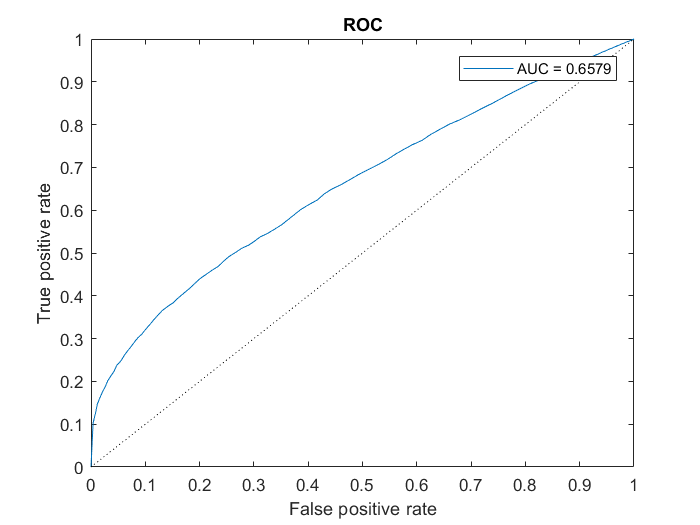
\includegraphics[width=\textwidth]{img/ROCchen.png}
    \end{subfigure}
    \hfill
    \begin{subfigure}[b]{0.5\textwidth}
        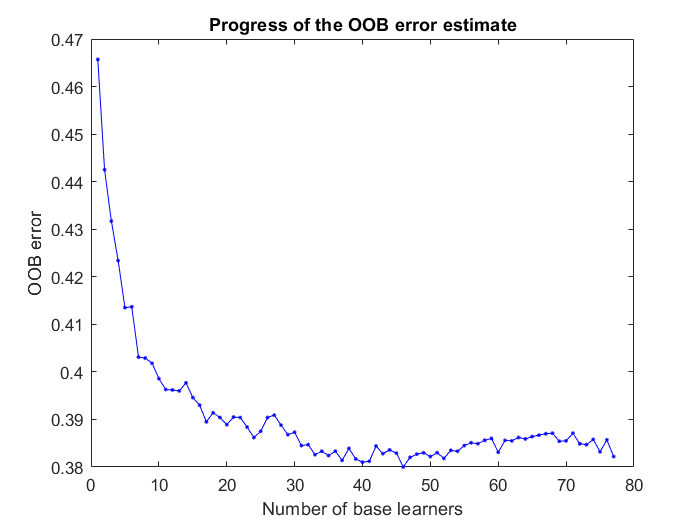
\includegraphics[width=\textwidth]{img/saturationchen.png}
    \end{subfigure}
    \caption{ROC and Search for subspace dimensionality}
\end{figure}
\begin{figure}[H]
    \begin{subfigure}[b]{0.5\textwidth}
        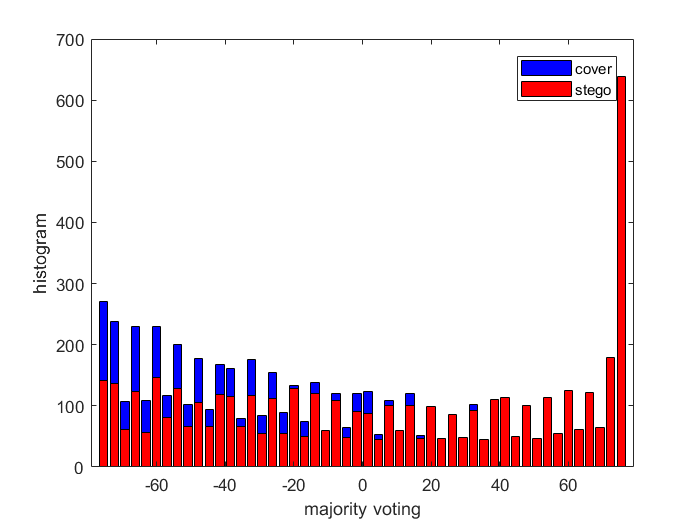
\includegraphics[width=\textwidth]{img/histochen.png}
    \end{subfigure}
    \hfill
    \begin{subfigure}[b]{0.5\textwidth}
        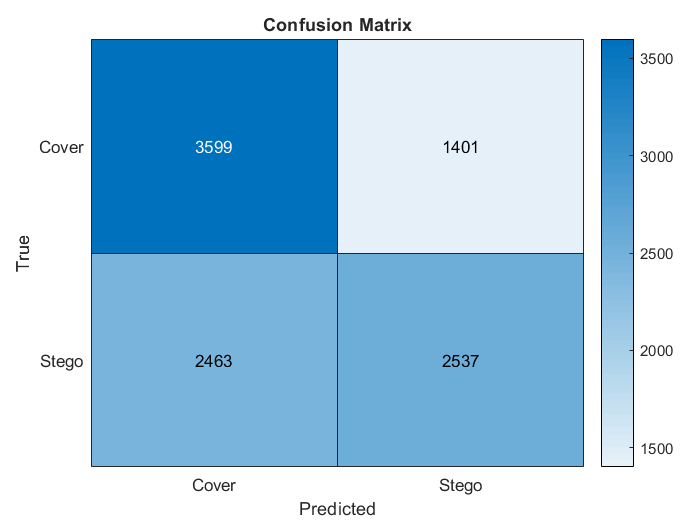
\includegraphics[width=\textwidth]{img/confusionChen.png}
    \end{subfigure}
    \caption{Histogram and Confusion Matrix}
\end{figure}

\section{Changing different parameters}
After comparing with two other features we decied to choose CC-C300 feature. To get the optimal result we trained our model with different value of dsub and number of base learner. The results are shown below:
\begin{table}[H]
    \begin{tabular}{|l|l|l|l|l|}
    \hline
    No of  Base Learner & Subspace size & Accuracy & Precision & Recall \\ \hline
    120                 & 800           & 0.6947   &           &        \\ \hline
    100                 & 1400          & 0.7045   &           &        \\ \hline
    160                 & 2600          & 0.7116   &           &        \\ \hline
    \end{tabular}
\end{table}
\begin{figure}[H]
    \begin{subfigure}[b]{0.5\textwidth}
        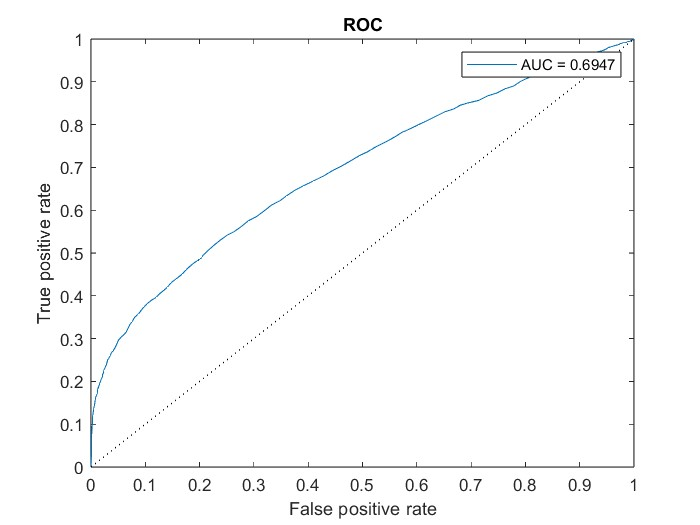
\includegraphics[width=\textwidth]{img/800/rocgray.jpg}
    \end{subfigure}
    \hfill
    \begin{subfigure}[b]{0.5\textwidth}
        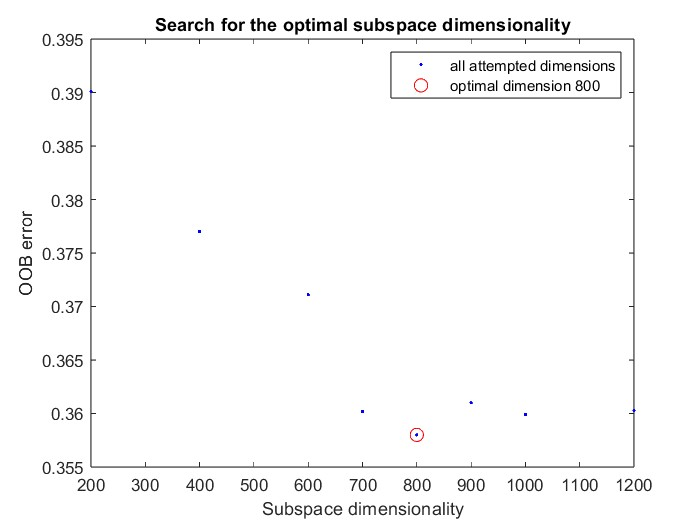
\includegraphics[width=\textwidth]{img/800/optimalgray.jpg}
    \end{subfigure}
    \caption{ROC and Search for subspace dimensionality [dsub=800]}
\end{figure}
\begin{figure}[H]
    \begin{subfigure}[b]{0.5\textwidth}
        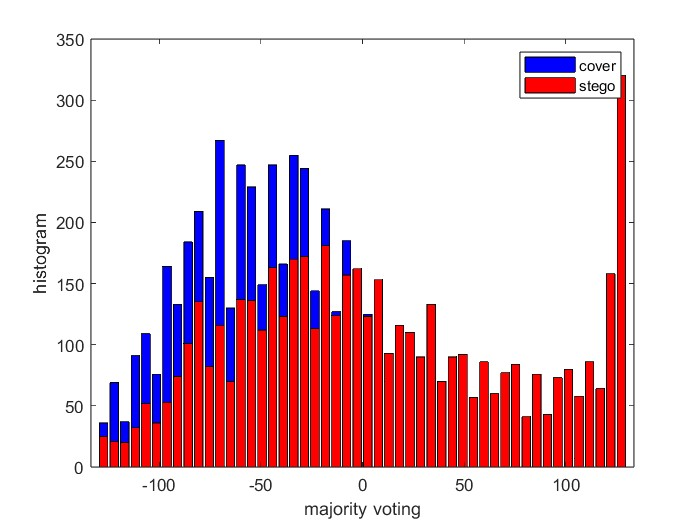
\includegraphics[width=\textwidth]{img/800/histogramgray.jpg}
    \end{subfigure}
    \hfill
    \begin{subfigure}[b]{0.5\textwidth}
        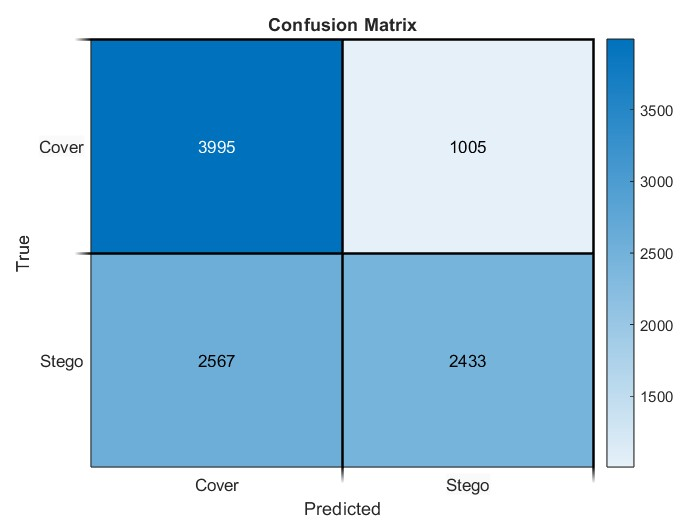
\includegraphics[width=\textwidth]{img/800/confusegray.jpg}
    \end{subfigure}
    \caption{Histogram and Confusion Matrix [dsub=800]}
\end{figure}

\begin{figure}[H]
    \begin{subfigure}[b]{0.5\textwidth}
        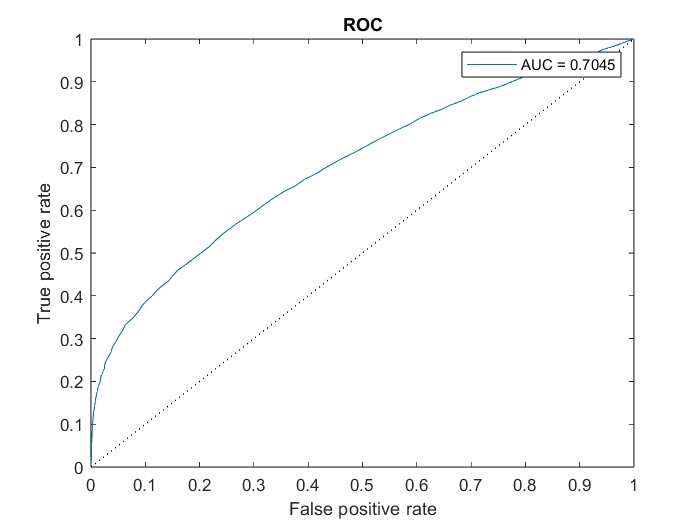
\includegraphics[width=\textwidth]{img/1400/gray1400roc.jpg}
    \end{subfigure}
    \hfill
    \begin{subfigure}[b]{0.5\textwidth}
        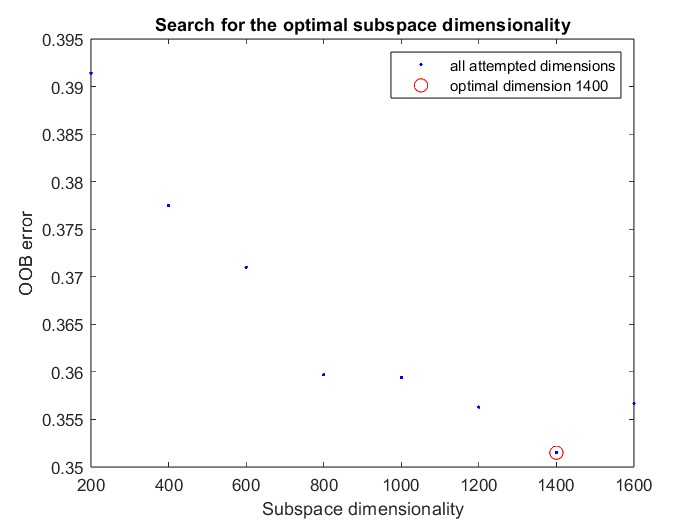
\includegraphics[width=\textwidth]{img/1400/gray1400iopti.jpg}
    \end{subfigure}
    \caption{ROC and Search for subspace dimensionality [dsub=1400]}
\end{figure}
\begin{figure}[H]
    \begin{subfigure}[b]{0.5\textwidth}
        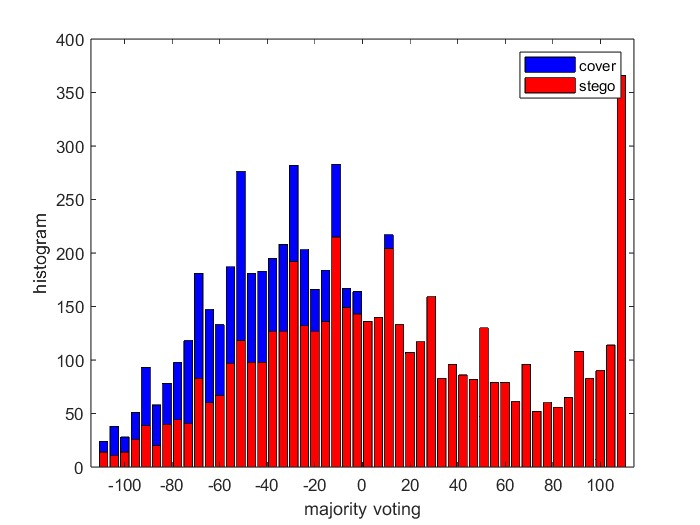
\includegraphics[width=\textwidth]{img/1400/gray1400histo.jpg}
    \end{subfigure}
    \hfill
    \begin{subfigure}[b]{0.5\textwidth}
        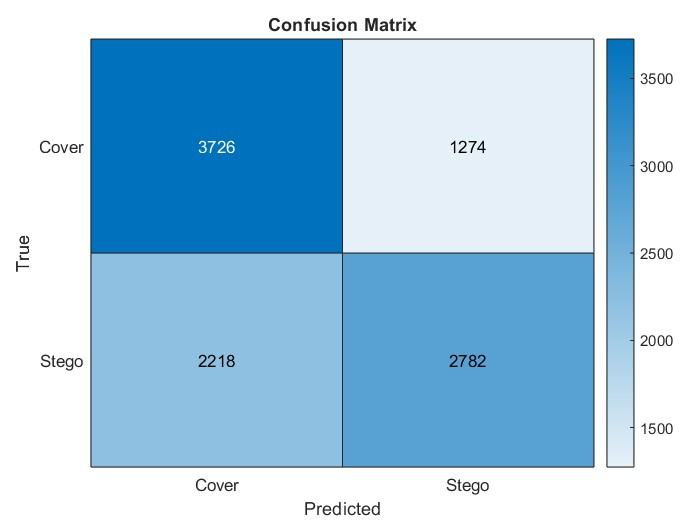
\includegraphics[width=\textwidth]{img/1400/gray1400confuse.jpg}
    \end{subfigure}
    \caption{Histogram and Confusion Matrix [dsub=1400]}
\end{figure}





In assessing classification methods, we experimented with using a Random Forest ensemble classifier in Python. The model's performance and accuracy closely matched those obtained using MATLAB.\\

The decision between MATLAB and Python as our primary platform was influenced by the availability of feature extraction tools. Since our feature extraction process was exclusive to MATLAB, we opted for it. Although it's possible to call MATLAB functions from Python, limitations such as version compatibility and slower execution using MATLAB Engine prompted us to stick with MATLAB for feature extraction.\\
TO call matlab from python it requires matlabengine. matlabengine is bla bla matlab ko version anusar python ko version vary garna parcha........ \\

For creating a demo, we investigated using MATLAB as a backend. It was possible but again it rquired matlabengine. so we used matlab app designer for the UI. mmatlab app designer is bla bla bla
k chutyo?
about matlab Engine
about matlab app designer
why matlab engine not used---------> slower
why matlab app designer used-----------> backend ma matlab engine use hune vayera 